\documentclass[a4paper]{article}
\usepackage[pdftex]{graphicx}
\usepackage[utf8]{inputenc}
\usepackage{enumerate}
\usepackage{amssymb}
\usepackage{icomma}
\usepackage{siunitx}
\sisetup{locale=DE}
\usepackage{tikz}
\usepackage{href-ul}
\hypersetup{
	colorlinks=true,
	linkcolor=blue,
	urlcolor=blue}
\usepackage{geometry}
\geometry{a4paper, top=15mm, left=15mm, right=15mm, bottom=15mm,
	headsep=10mm, footskip=12mm}

\begin{document}
	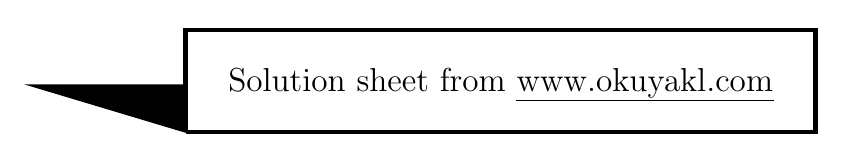
\begin{tikzpicture}(10,3)
		\draw[ultra thick](2,0) --(10,0) -- (10,1.3) --(2,1.3) -- (2,0);
		\draw[fill=black](2,0)-- (0,.6) -- (2,.6) -- (2,0);
		\node at (6,.6) {\large Solution sheet from \href{http://www.okuyakl.com}{www.okuyakl.com}};
	\end{tikzpicture}
	\vspace{0.5 cm}
	
	\noindent{\bf Task 1.}\\
	
	
	\renewcommand{\arraystretch}{1.8}
	\begin{tabular}{|p{1.7 cm}|p{1.7 cm}|p{1.7 cm}|p{1.7 cm}|p{1.7 cm}|p{1.7 cm}|p{1.7 cm}|p {1.7cm}|}
		\hline
		Cloth & Wood & Lead & Water & Air & Edible Oil & Gold & Aluminum \\
		\hline
		State & solid & solid & liquid & gaseous & liquid & solid & solid \\
		\hline
		Example & Building Block & Fishing Lead & Bottle & Balloon & Bottle & Ingots & Sharpener\\
		\hline
		Mass & $\SI{35}{\gram}$ & $\SI{5.0}{\gram}$ & $\SI{1.5}{\kilo\gram}$ & $\SI{5, 2}{\gram}$ & $\SI{0.63}{\kilogram}$ & $\SI{12.4}{\kilogram}$ &$\SI{4.3}{\gram}$ \\
		\hline
		Volume &$\SI{50}{\centi\meter^3}$ & $\SI{0.44}{\centi\meter^3}$ &$\SI{1.5}{\deci\meter^ 3}$ & $\SI{4.0}{\deci\meter^3}$ & $\SI{0.7}{\deci\meter^3 }$ &$\SI{0.64}{\deci\meter^3}$ & $\SI{1,6}{\centi\meter^3}$ \\
		\hline
		Density &$\SI{0.7}{\gram\over{\centi\meter^3}}$ &$\SI{11.3}{\gram\over{\centi\meter^3}}$ &$\SI{1.0}{\gram\over{\centi\meter^3}}$ &$\SI{1.3}{\gram\over{\deci\meter^3}}$ &$\SI{0.9}{\ gram\over{\centi\meter^3}}$ &$\SI{19,3}{\gram\over{\centi\meter^3}}$ &$\SI{2,7}{\gram\over{\centi\meter^3}}$ \\
		\hline
	\end{tabular}
	\vspace{0.5 cm}
	
	\begin{tabular}{|p{1.4 cm}|p{1.4 cm}|p{1.5 cm}|p{1.8 cm}|p{1.7 cm}|p{2.0 cm}|p{2.1 cm}|p {1.7cm}|}
		\hline
		Fabric & Cork & Iron & Styrofoam & Hydrogen & Iridium & Mercury & Polyethylene \\
		\hline
		State & solid & solid & solid & gaseous & solid & liquid & solid \\
		\hline
		Example & cork & key & insulation board & balloon & original kilogram & thermometer & dice\\
		\hline
		Mass &$\SI{1.9}{\gram}$ &$\SI{8.5}{\gram}$ & $\SI{150}{\gram}$ & $\SI{0.41} {\gram}$ & $\SI{1,0}{\kilogram}$ & $\SI{0.67}{\gram}$ & $\SI{3,1}{\gram}$\\
		\hline
		Volume &$\SI{6.2}{\centi\meter^3}$ & $\SI{1.1}{\centi\meter^3}$ & $\SI{5.0}{\deci\meter^3}$ & $\SI{4.5}{\deci \meter^3}$ & $\SI{45}{\centi \meter^3}$ &$\SI{0.05}{\centi\meter^3}$ &$\SI{3,3}{\centi\meter^3}$ \\
		\hline
		Density &$\SI{0.3}{\gram\over{\centi\meter^3}}$ &$\SI{7.7}{\gram\over{\centi\meter^3}}$ &$\SI{ 0.03}{\gram\over{\centi\meter^3}}$ &$\SI{90}{\gram\over\meter^3}$ &$\SI{22.4}{\gram\over\ centi\meter^3}$ &$\SI{13.5}{\gram\over{\centi\meter^3}}$ &$\SI{0.95}{\gram\over{\centi\meter^3}} $\\
		\hline
	\end{tabular}
	\vspace{0.5 cm}
	
	\noindent{\bf Task 2.}\\
	Lightest substance: hydrogen; Heaviest material: Iridium
	\vspace{0.5 cm}
	
	\noindent{\bf Task 3.}\\
	The surrounding air is specifically heavier than the hydrogen balloon, which is why it experiences a buoyant force
	\vspace{0.5 cm}
	
	\noindent{\bf Task 4. a)}\\
	\renewcommand{\arraystretch}{2}
	\begin{tabular}{|p{3 cm}|p{12.5 cm}|}
		\hline
		Floats in & fabric\\
		\hline
		Cooking oil & wood, cork, styrofoam\\
		\hline
		Water & wood, cork, styrofoam, polyethylene \\
		\hline
		Mercury & wood, cork, Styrofoam, polyethylene, lead, iron, aluminum\\
		\hline
	\end{tabular}
	\vspace{0.5 cm}
	
	\noindent{\bf Task 4. b)}\\
	Polyethylene is specifically heavier than cooking oil but lighter than water
	\vspace{0.5 cm}
	
	\noindent{\bf Task 4. c)}\\
	Gold, iridium.
	
	\begin{center}
		\includegraphics[width=7 cm]{../../viecher/eendcomic.pdf}
		
		Here you can go back to the \href{https://www.okuyakl.de/phys/p7dihL073/ae073.pdf}{task sheet}
	\end{center}
	
	
	
\end{document}